\chapter{State of the Art}
\lhead{\chaptername~\thechapter. \emph{State of the Art}}
\label{ch:state_of_the_art}
%
In this chapter, we define formally the VO problem, we describe a generic perspective SfM pipeline, 
and then we introduce the main challenges and issues when employing full spherical cameras for VO.
During this description we refer, time by time, to the related state of the art algorithms/methods.

%
% Start of sections from intro

\section{SfM, VO, and SLAM}
SfM is a long studied topic in computer vision. Starting from an input of photographs taken by one or multiple cameras, SfM's main goal is to compute the cameras' poses and to reconstruct the 3D environment's geometry captured by those cameras~\cite{szeliski2010computer}.
%
Some of the first works are the paper by Longuet-Higgins~\cite{longuet1981computer}, whose equations are fundamental in epipolar geometry, and the paper by Tomasi et al.~\cite{tomasi1992shape}, who used orthographic photographs to estimate the shape of a 3D object.
%
SfM is a general term, and it also includes \textit{visual odometry} (VO). This is the problem of recovering the motion of an agent equipped with a camera rig in a 3D environment. Typically, VO deals with an ordered set of images such as video sequences, and it uses them to compute the egomotion in real-time. Nister et al.\cite{nister2004visual} introduced the term \textit{visual odometry} for the first time.

Another field of robotic/computer vision research that is very close to VO is \textit{simultaneous localization and mapping} (SLAM). SLAM targets the problem of creating a map of the environment where a camera equipped agent navigates and simultaneously estimating its path. Scaramuzza\cite{scaramuzzaVisualOdometryI} pointed out that while VO is more focused on local motion estimation, SLAM's goal is to obtain a global consistent estimation of the agent movements.
%
In order to reduce error, SLAM keeps track of the visited path and can decide when the agent has come back to a previously visited location. This extra step in SLAM's pipeline is called \textit{loop closure} and provides an additional constraint used to reduce errors in both the agent's path and 
environment reconstruction. Durrant-White et al.\cite{durrant1996localization} firstly introduced the term SLAM.
 
\section{Densification: from Sparse to Dense Point Cloud}
A sparse point cloud is the product of most SfM pipelines; some keypoints are tracked in each photograph and are then used by the motion estimation algorithm. These keypoints are triangulated and their corresponding world points are available during egomotion estimation.
%
A set of triangulated keypoints is a sparse point cloud around the camera's path. This set provides a first approximation of the environment reconstruction.
Typically, starting from this information, it is possible to obtain a complete reconstruction of the 3D environment by applying
a so-called \emph{Multi View Stereo} algorithm. The goal of Multi View Stereo\cite{seitz2006comparison} is to reconstruct a complete
3D object model from a collection of images taken from known camera poses.
Many of these algorithms obtain a dense point cloud starting from the sparse reconstruction, and then 
estimate the final surface according to this dense point set.

Our approach consists in densify the point cloud by computing, for each pair of consecutive images, 
a depth map. These depth maps are merged to obtain a dense set of reconstructed points. At this point the 
surface can be reconstructed by applying a surface fitting algorithm such as the standard Poisson reconstruction\todo{??CITARE??}.
A depth map consists in associating a value of depth for each pixels of the images pair.
The depth map estimation involves the calculation of a \emph{disparity map} from the images pair. 
This is a map of the distance in pixels from a point in a reference image and its corresponding point in the 
other image. Higher is the disparity of a given pixel, higher is the parallax and hence the depth of that pixel. 
The map is usually computed based on some kind of similarity 
metric such as \emph{sum of absolute distances} (SAD), 
\emph{sum of squared distances} (SSD), 
\emph{normalized cross correlation} (NCC), etc. These provides a way to 
compute the corresponding point in the second image, thus enabling the 
computation of the disparity for every point in the reference image.
Figure~\ref{fig:disparity_example} shows an example of disparity map.

\begin{figure}[h]
	\centering
	\begin{subfigure}{0.4\textwidth}
		\centering
		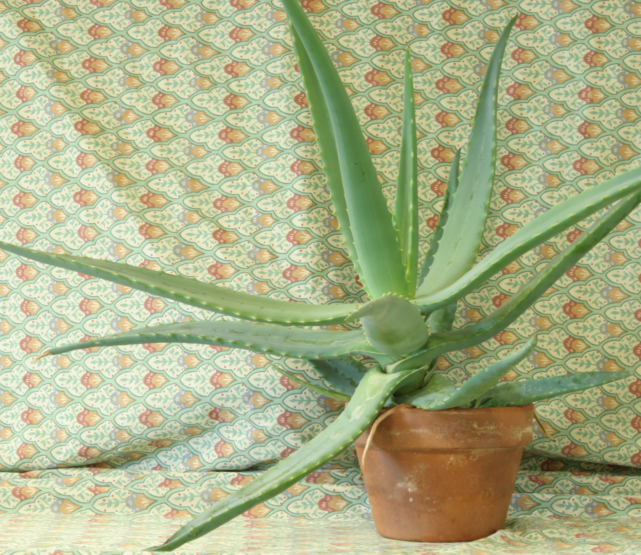
\includegraphics[width=0.7\textwidth]{img/aloe_view1}
	\end{subfigure}
	\begin{subfigure}{0.4\textwidth}
		\centering
		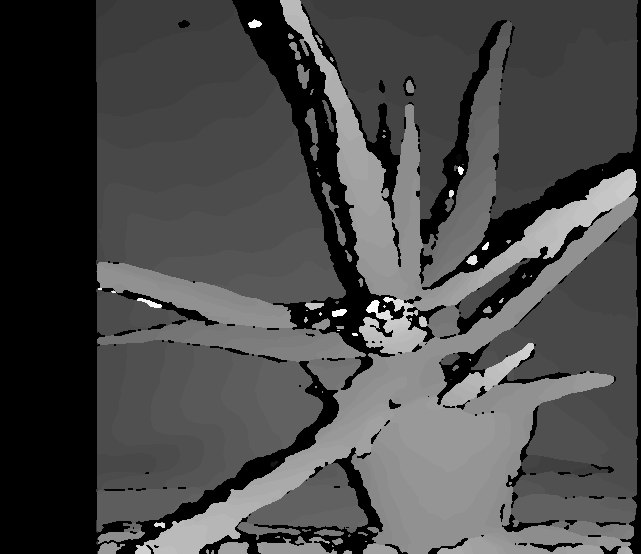
\includegraphics[width=0.7\textwidth]{img/aloe_disparity}
	\end{subfigure}
	\caption{\label{fig:disparity_example}An example of disparity map from the
	Middlebury dataset~\cite{hirschmuller2007evaluation}}
\end{figure}

\section{Omnidirectional and Full Spherical Cameras}
\label{sec:cameraclassification}
Omnidirectional cameras are characterized by wide field of view. Indeed, many of this kind of devices can take pictures with a 180\degree view angle or even wider.

There are several ways to obtain panoramic images, they include:
\begin{itemize}
	\item perspective cameras and image stitching;
	\item catadioptric cameras;
	\item dioptric cameras;
	\item hybrid approaches.
\end{itemize}

Perspective cameras can take panoramic pictures with the aid of software stitching. As the first step, we take several photographs with many cameras or by simply moving the same camera in order to cover most of a scene. Then, a stitching software merges all images into a single one. To use a traditional camera and a stitching software is the cheapest way to obtain panoramic images because it does not need any kind of specialized hardware. However, this process is cumbersome (a lot of manual work is required). Note that some smart-phones provide built-in camera 360\degree acquisition modes, but the final quality may be not satisfactory due to alignment artifacts.
An example for this approach is the Hugin Panorama Photo Stitcher 
\cite{hugin_photostitcher}, an open source software for merging several 
perspective images in a single panoramic picture.
The SpheroCam\texttrademark by SPHERON-VR AG\texttrademark~\cite{spheronvr}
is an alternative to 
the latter approach to panoramic images; it uses a specialized hardware composed
of a wide angle lenses equipped camera mounted on a rotating support, which rotates around the optical center of the camera. Therefore, this camera can capture high quality full spherical and it addresses the professional fields of geographical analysis, forensic investigation, cultural heritage, etc.

A catadioptric camera can be obtained by coupling a perspective camera and a mirror, which is mounted in front of camera. Such setup takes a picture of the mirror that reflects the surrounding. The mirror of a catadioptric system may have several shapes. The most common one is the hyperbolic profile that creates a single center of projection for every ray coming to the mirror.

A traditional camera can also be adapted to work as a panoramic one by adding a fisheye lens capable of refracting lights from wide angle towards the image sensor. These setups are called dioptric cameras.

Apart of perspective cameras coupled with stitching software, none of the previous approaches can take full spherical panoramic photographs. Moreover, full spherical videos cannot be shot with perspective cameras either.

The last approach, an hybrid one, exploits several sensors using fisheye lenses and software stitching to capture full spherical panoramic images in a single shot. This enables full spherical video capturing as well. The camera (that is composed of several image sensors) take multiple overlapping pictures simultaneously. Then, an on camera stitching software composes the data in a single image.

In all our experiments we used the Ricoh Theta S camera that is a hybrid full spherical camera composed of two fisheye lenses with a FOV greater than 180\degree; see Figure~\ref{fig:ricoh_theta}.
%
%
% end of sections from intro

\section{VO Problem}
\label{sec:vo_problem}
As we described in the previous chapter, the VO's goal is to recover the 
camera trajectory while it is moving in the environment. Following Scaramuzza and Fraundorfer\cite{scaramuzzaVisualOdometryI},
we introduce the notations that we are going to use for the rest of this work.
%
Let first assume time is sampled in a sequence of time instants \(k\); 
\(I_{0:(n - 1)} \) is the set of $n$ input frames, where \(I_{k}\) is a picture taken by 
the camera at time \(k\). We define \(C_{0:(n-1)}\) as the set of camera 
positions such that \(C_k\) is the position at the \(k\)-th time.
If we call \(T_k\) the rigid body transformation of the camera between two
consecutive time instants (i.e., $k-1$ and $k$), then we have the following relation:
%
\begin{equation}
	C_k = C_{k-1} T_k
	\label{eq:motion_composition}
\end{equation}
%
\noindent where \(T_k\) is defined as
%
\begin{equation*}
	T_k =
	\begin{bmatrix}
	R_k & \myvec{t}_k \\
	0 & 1
	\end{bmatrix} \text{,}
\end{equation*}
%
\noindent where $R_k$ is a 3-by-3 rotation matrix (i.e., the rotation of the camera at time $k$),
$\myvec{t}_k$ is a column vector (i.e., translation of the camera at time $k$).
Therefore, the goal of VO is to estimate both $R_k$ and $t_k$ for each time 
$k$ and to compute each $C_k$ accordingly to equation~\ref{eq:motion_composition}. Note that the initial position $C_0$ can be set arbitrarily.

Equation~\ref{eq:motion_composition} is the core of VO, that allows us to compute the camera local movement. Therefore, we can estimate its location in every instant of time. However, the equation above contains also the most insidious practical challenge of VO; i.e., the error accumulation phenomenon known as \emph{drift}.
Every new position $C_k$ can introduce an error factor that affects the next 
computations. The results is a global error that grows as the number of 
estimations increases.
%
Since early works such as Harris et al.\cite{harris19883d} and Moravec\cite{moravec1980obstacle}, the VO research community has focused on error minimization techniques to reduce drift.
This tackles the precise estimation problem either by employing more accurate
local motion estimation and by introducing an optimization step to refine 
camera locations.
The set of techniques for reducing the drift (after the camera poses are computed) is typically called \emph{bundle adjustment}~\cite{triggs1999bundle}.

\section{Perspective SfM}
The SfM literature is vast, but most of the approaches present pipelines similar to the one in 
Fig.~\ref{fig:block_diagram}.
The main steps are: to compute the relative motion for each image
pair, to compose these motions for obtaining the absolute camera position and 
orientation, and to run a drift reduction procedure.
%
The differences are in the type of input data, motion estimation algorithm,
optimization procedure and additional constraints considered.
For generic SfM researches, the input data is a set of traditional pictures of 
the same environment from different point of view. The pictures can be taken by 
different cameras with unknown parameters and in different time instants.
%
\begin{figure}
	\centering
	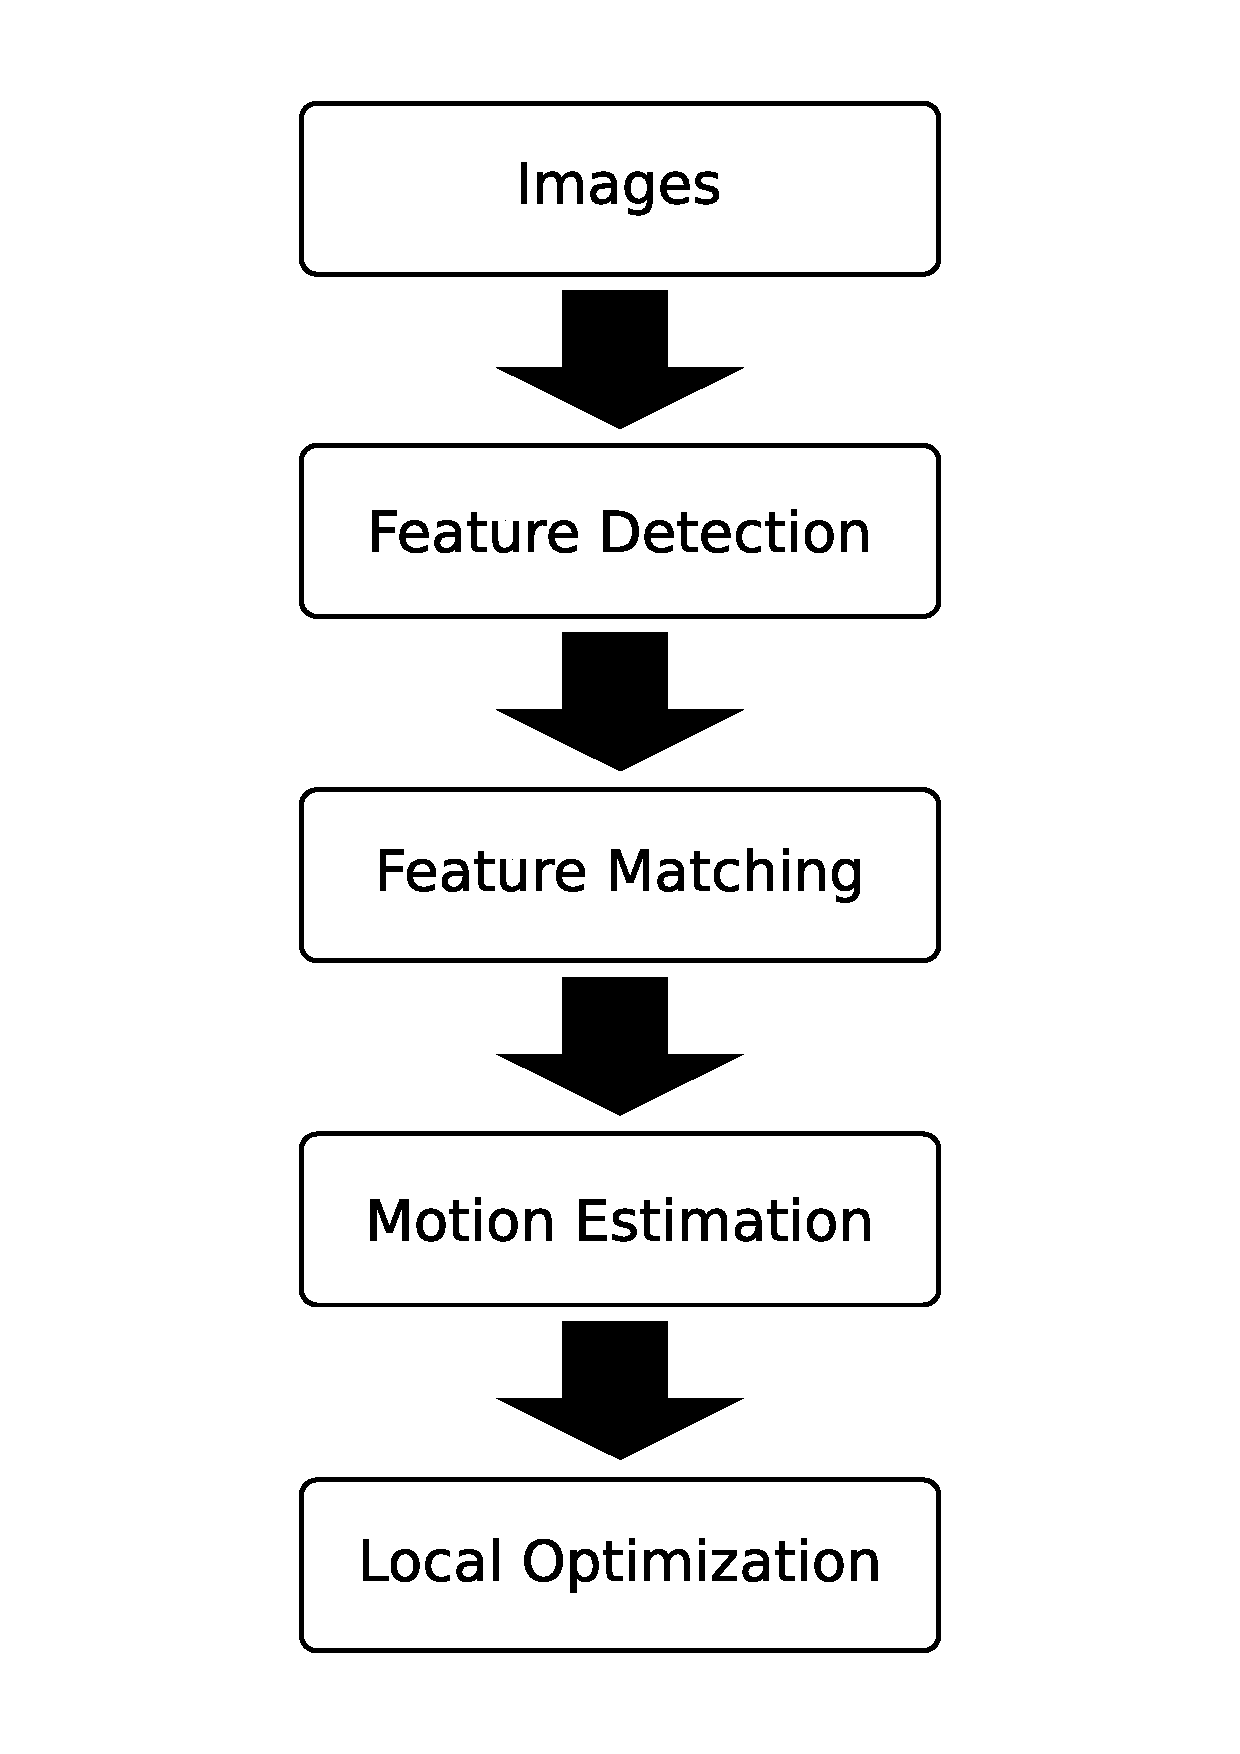
\includegraphics[width=\linewidth]{img/block_diagram.pdf}
	\caption{Perspective SfM pipeline block diagram.}
	\label{fig:block_diagram}
\end{figure}

\textit{Visual Odometry} is based on SfM techniques, 
in this case, the input data is usually a sequence 
of images from a video stream. The image capturing devices can vary:
Moravec used a sliding camera that could capture stereo images~\cite{moravec1980obstacle} while Matthies et al. equipped their robot with
an actual stereo rig~\cite{matthies1987error};
in~\cite{nister2004visual} Nister et al used a single perspective camera.
The computer vision literature refers to the
single camera studies case with the term \textit{monocular VO} while it uses \textit{stereo VO} to describe the work done with stereo equipment.

Even though perspective cameras have been the first choice in many studies, 
the researchers used other devices, like the ones described in 
\ref{sec:cameraclassification}.

We use the terms \textit{perspective} or \textit{traditional SfM} to describe 
SfM pipelines designed for perspective cameras.

A great resource about the state of the art for VO and SfM is the work by Scaramuzza and Fraundorfer,  
\cite{scaramuzzaVisualOdometryI, scaramuzzaVisualOdometryII}.

\subsection{Motion Estimation}
\label{subsec:motion_estimation}
We use the term local motion to indicate the camera movement between two 
consecutive images while, on the other hand, we define global motion as
the overall camera's path.
The local motion estimation step is fundamental in a SfM pipeline, its goal is 
to find the rigid body transformation composed of $R_k$ and $t_k$ as we 
described in Section~\ref{sec:vo_problem}.
All the local motion estimation methods described in the literature so far are 
based on the correspondences found in two consecutive images but, depending on the
specific camera rig (stereo imaging systems or monocular), the type of 
correspondences and their matching procedure, we may have several choices for
the actual way to estimate local motion.
There are two main families of point matching algorithms: \textit{feature-based}
and \textit{appearance-based} (also known as \textit{global-methods}).
While the former ones utilize repeatable features 
matching between the images, the latter rely on pixel's intensity information; 
they are simpler but also slower. Most of the 
most recent VO pipelines use feature-based methods because of
their speed and robustness.
A VO implementation that employs intensity based techniques is 
\cite{nister2004visual}, while~\cite{makadia2007correspondence} is an example 
of featureless motion estimation method.

Each of the feature points found by the motion estimation phase can be 
either a 3D world-point feature or a 2D image-point one,
therefore, there are three possible combinations that provides just as many 
different matching and motion-estimation procedures:
\begin{itemize}
	\item 2D-to-2D: both feature sets are composed of image points.
The matching metric can be a simple euclidean distance between feature 
descriptors and the motion estimation can be solved by estimating the 
\textit{essential matrix} (see section~\ref{subsec:essential_matrix} for 
details);
	\item 3D-to-3D: both feature sets contain world-points features and motion
estimation is performed by solving an alignment problem;
	\item 3D-to-2D: the previous image's feature set is composed of world points while
the current one's feature set contains their projections. In this case, the motion 
is estimated by solving a problem called Perspective-n-Points (\textit{PnP}).
\end{itemize}
Since the second and third approaches deal with 3D points, they are usually 
best suited for stereo rig (especially the 3D-to-3D case).
Obviously, we can still use the 3D-to-2D approach in the monocular VO case by simply 
triangulating corresponding 2D image features in consecutive frames.
In fact, in order to obtain the first 3D feature set,
we can compute the relative motion between the first two images with 
the 2D-to-2D techniques and then obtain the rest of the camera's path,
as we said, by solving the \textit{PnP} problem.
%
\begin{figure}[ht]
	\centering
	\begin{subfigure}{\textwidth}
		\centering
		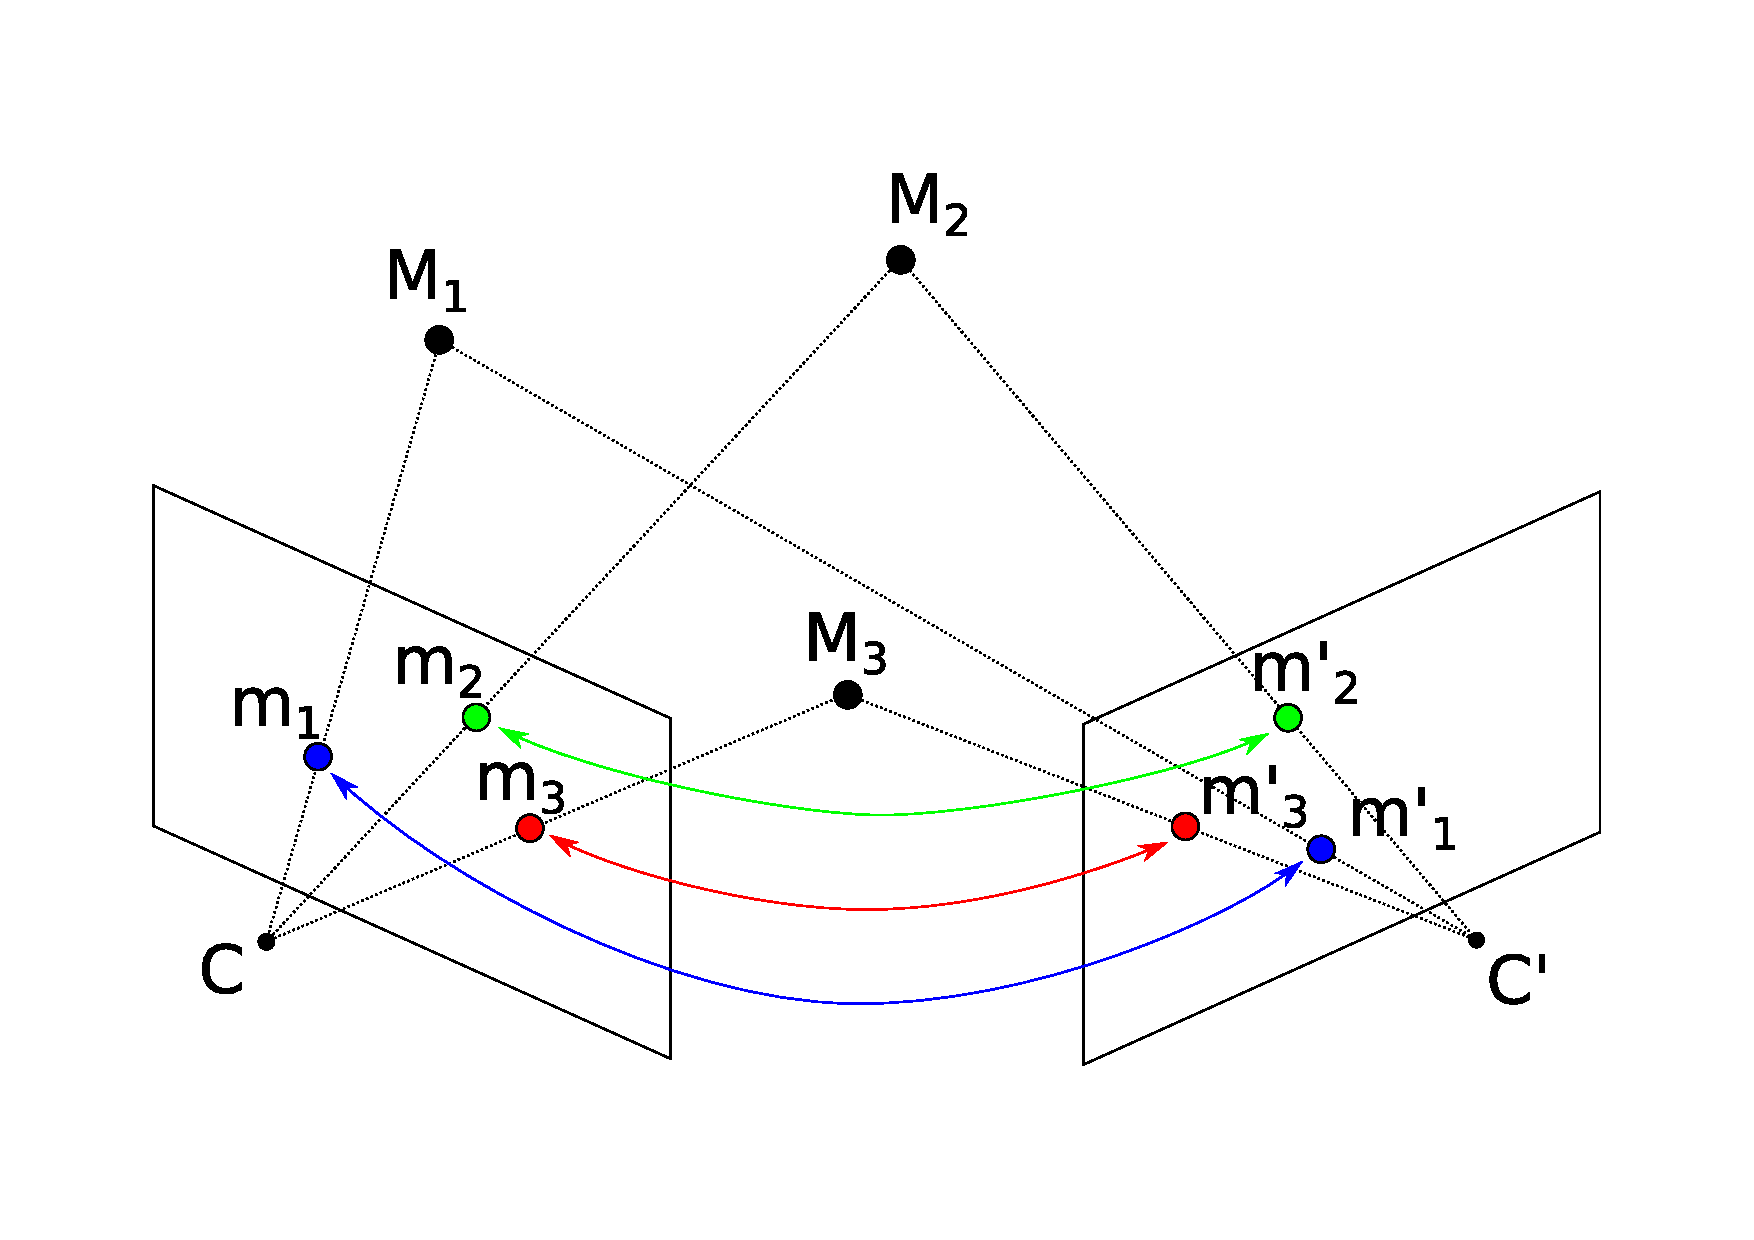
\includegraphics[width=0.5\linewidth]{img/correspondence1.pdf}
		\caption{2D-to-2D.}
        \label{fig:approach1}
	\end{subfigure}
    %
	\begin{subfigure}{\textwidth}
		\centering
		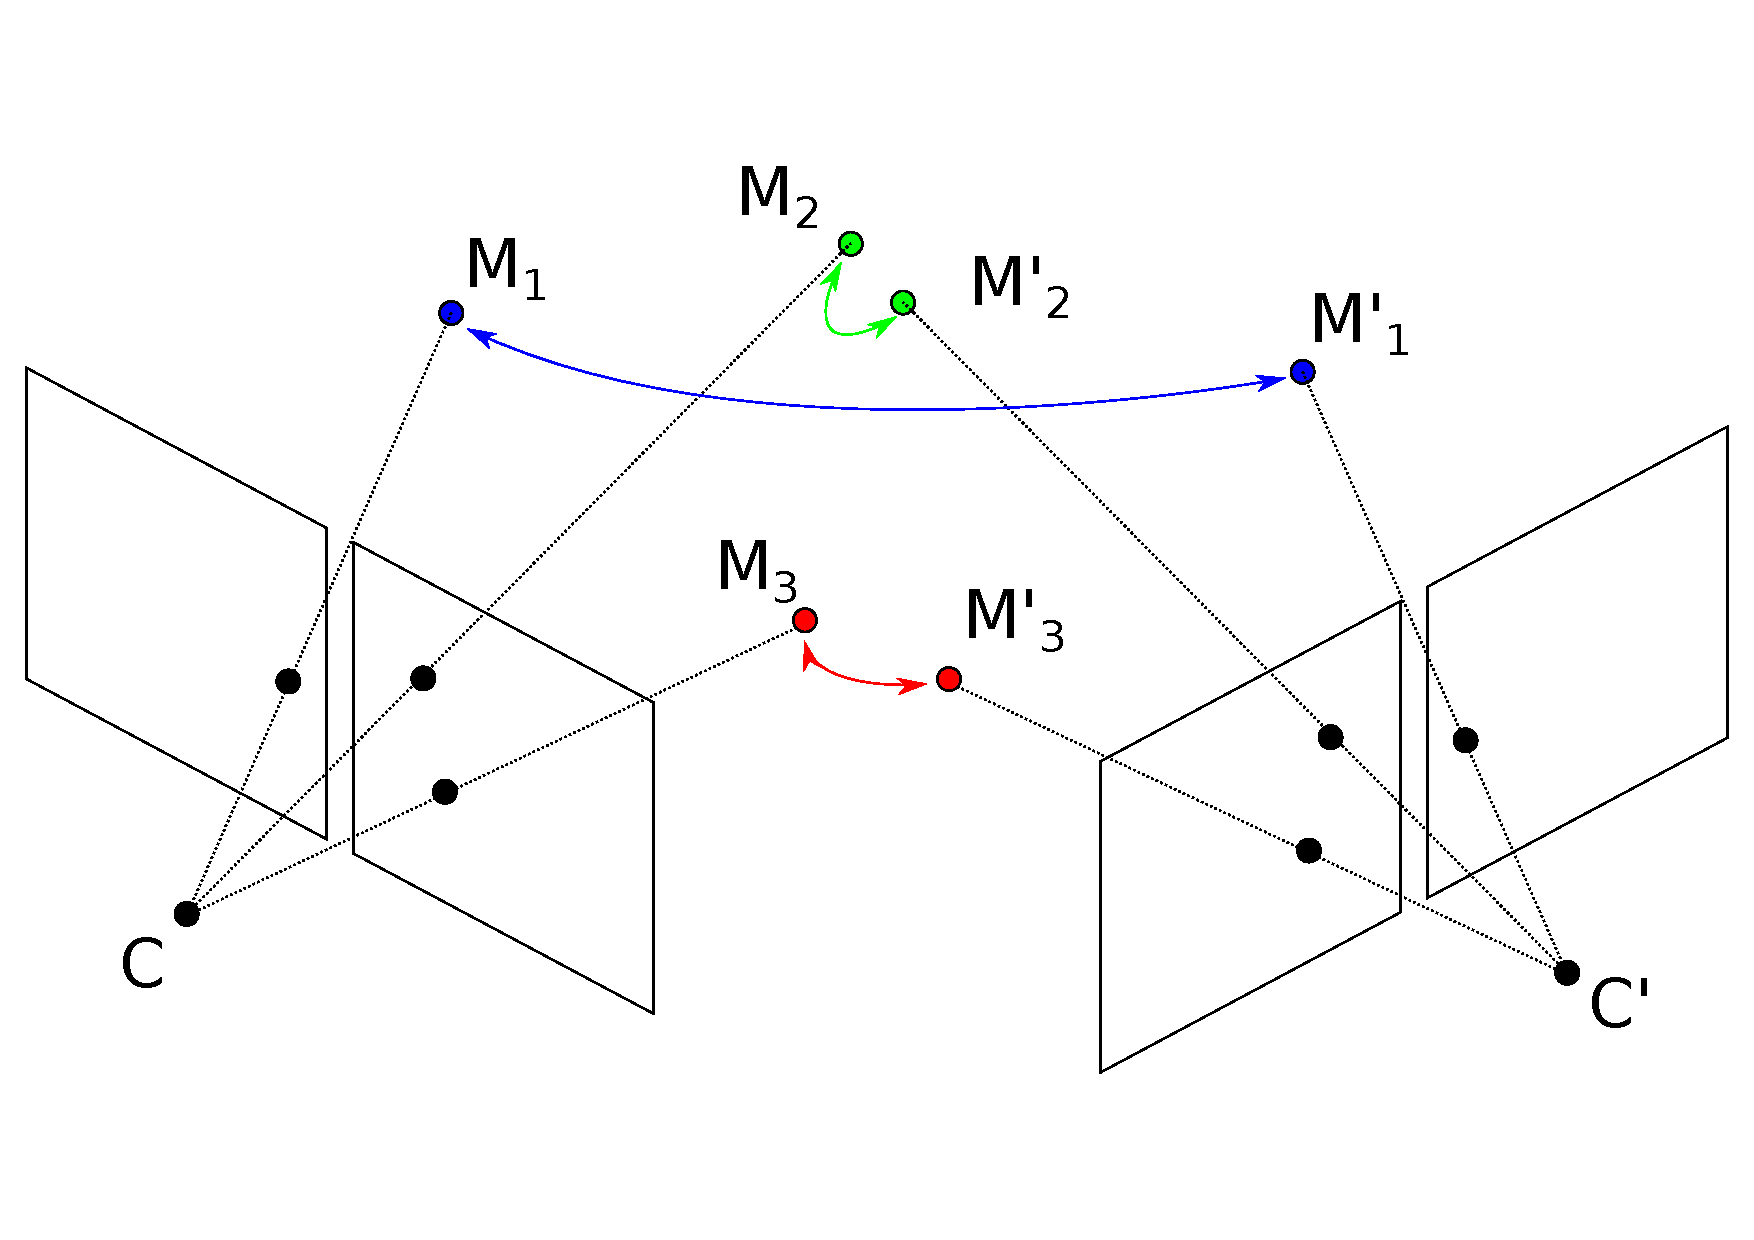
\includegraphics[width=0.5\linewidth]{img/correspondence3.pdf}
		\caption{3D-to-3D.}
        \label{fig:approach2}
	\end{subfigure}
    %
	\begin{subfigure}{\textwidth}
		\centering
		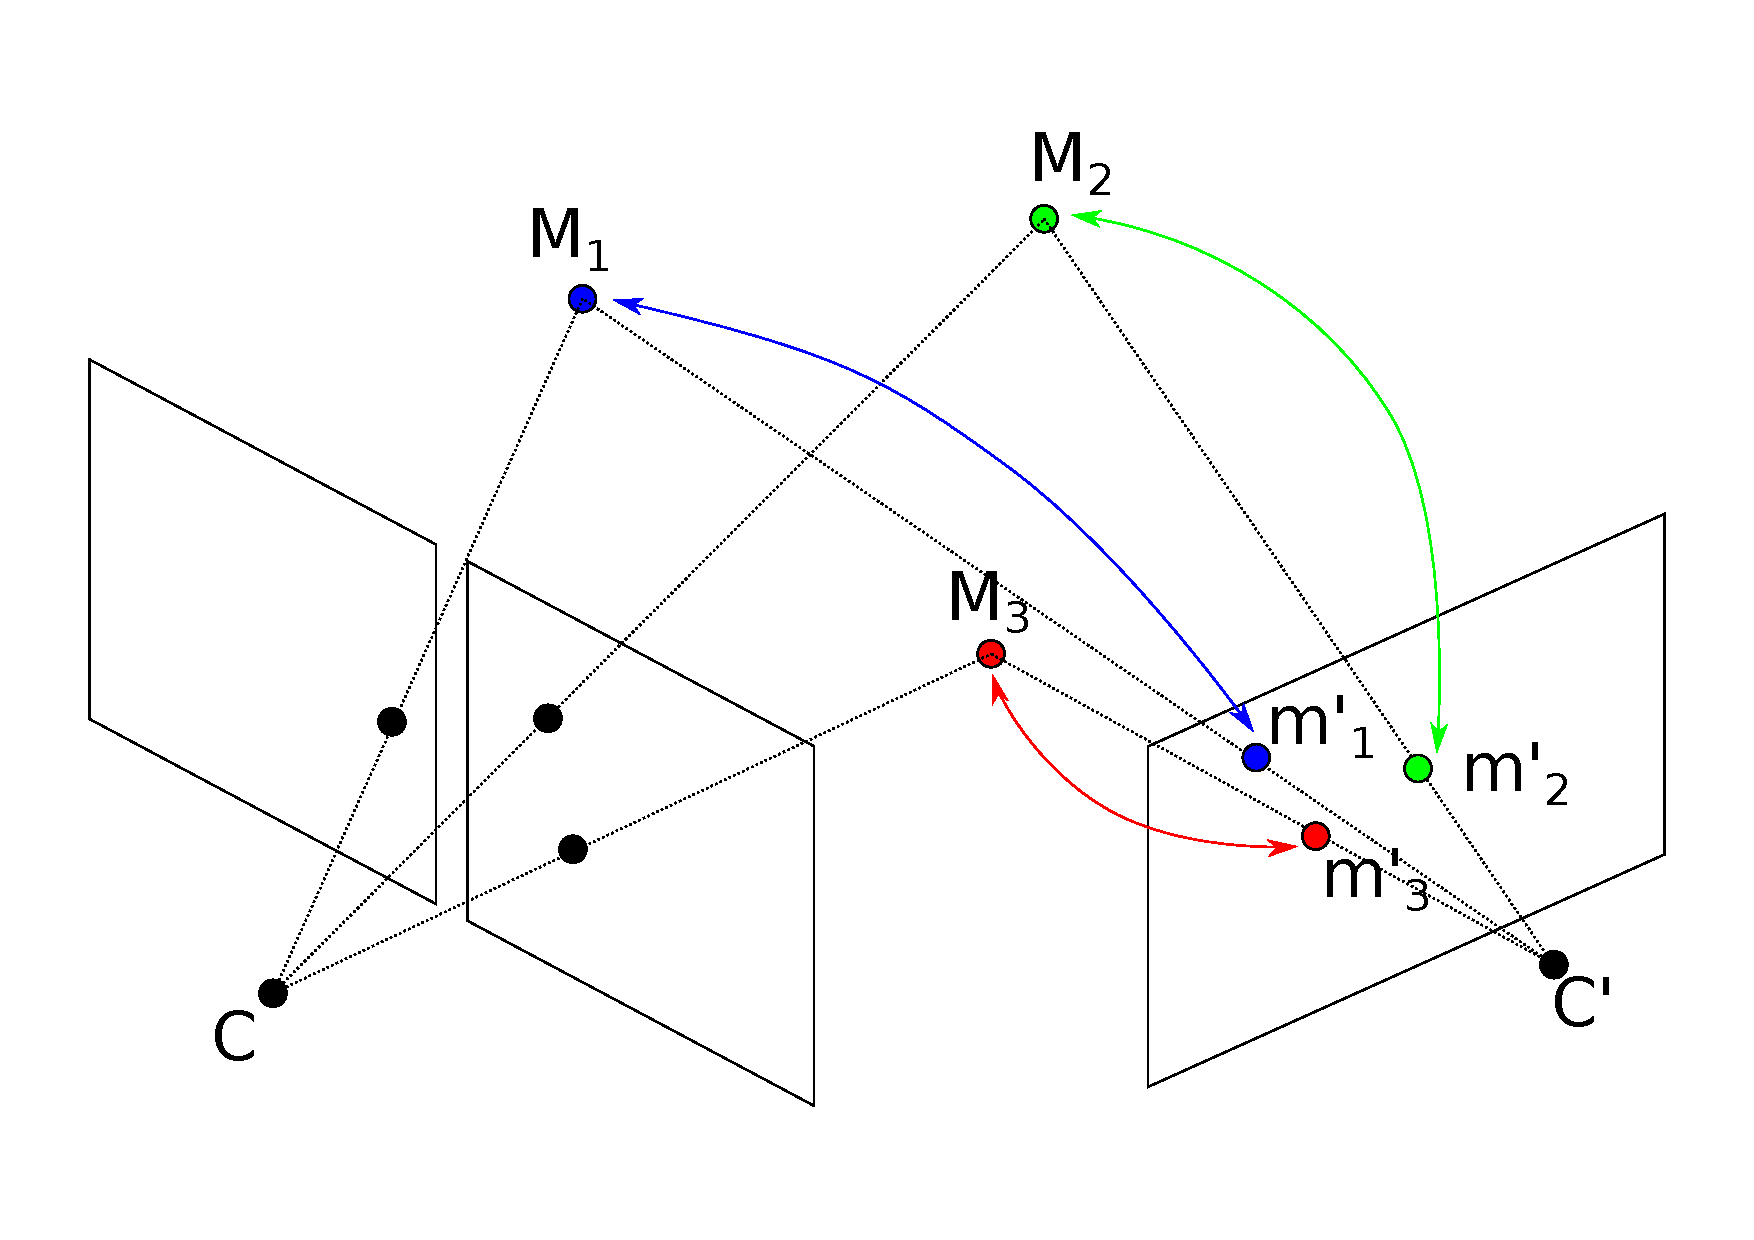
\includegraphics[width=0.5\linewidth]{img/correspondence2.pdf}
		\caption{3D-to-2D.}
        \label{fig:approach3}
	\end{subfigure}
    %
	\caption{Representation of the feature matching step for motion estimation.
	Uppercase letters indicates 3D points while lowercase letters are 2D image
	points; the new pose is $C'$. Note the stereo rigs in (b) and 
	(c) to highlight the need for triangulated world points with these 
	approaches.}
    \label{fig:poseestimation_approaches}
\end{figure}

\subsubsection{Essential Matrix}
\label{subsec:essential_matrix}
The essential matrix $E$ is defined as
%
\begin{equation}
\label{eq:epipolar_equation}
	\myvec{p}^{\prime\top} E \myvec{p} = 0 \text{,}
\end{equation}
%
\noindent where $\mathbf{p}$ and $\mathbf{p}^\prime$ are, respectively, the normalized corresponding 
feature coordinates in image $I_{k-1}$ and $I_{k}$. The normalized coordinates are defined as
%
\begin{equation}
	\mathbf{p} = K^{-1} \mathbf{m} \text{,}
\end{equation}
%
\noindent where $K$ is the intrinsic parameter matrix, and $\mathbf{m}$ is an
image point.
The essential matrix contains the geometric information that describe the 
relative location of a camera respect to another one up to an unknown scale factor 
for the translation vector. In particular, we have:
%$
\begin{equation*}
	E_k = \lambda \hat{t}_kR_k \text{,}
\end{equation*}
%$
\noindent where $\lambda$ is an unknown scale factor, and $\hat{t}_k$ is 
the skew-symmetric form for the cross product of vector $t_k$.
In order to extract the local motion given the two set of corresponding features
in two consecutive images, we have to estimate the essential matrix and then 
extract the rigid body transformation out of it.
For the $E$ estimation part we can employ the Longuet-Higgins' 8-points 
algorithm~\cite{longuet1981computer}: the equation~\ref{eq:epipolar_equation} 
provides a constraint we
can exploit for computation, in fact, for each correspondence, we can rewrite 
the equation as
%
\begin{equation*}
	\begin{bmatrix}
		p_1p^\prime_1 & 
        p^\prime_1p_2 & 
        p^\prime_1 & 
        p_1p^\prime_2 & 
        p_2p^\prime_2 & 
        p^\prime_2 & 
        p_1 & p_2 & 
        1
	\end{bmatrix} 
    \cdot
	E = 0	\text{.}
\end{equation*}
%
To find the nine unknowns, we need 8 non-coplanar feature matches that provide as many 
independent equations. In practice, we use more than 8 points, i.e., we obtain a overdetermined 
system that we solve in the least square sense.

Once we estimate $E$, there are four possible cases for the relative 
position of the two cameras and each world points. We are interested in the one
that presents both cameras facing toward the triangulated world point; i.e., this point has to be in front of both cameras. We can determine the correct configuration among the four by testing each of them using triangulation.

\subsubsection{Relative Scale}
As we have already pointed out in the previous section, every monocular SfM 
pipeline that works with 2D-to-2D feature correspondences can estimate the 
local motion up to an unknown scale factor. There is no way to extract 
the translation magnitude from two sets of features (it is still possible 
to recover the reconstruction scale if we are given some world measure of the
environment).
Therefore, if we can not derive the local translation length with some other
non visual techniques (such as wheel odometry, GPS, accelerometer, etc.).
We have to keep this unknown scale for the motion estimation and 
environment reconstruction.

On the other hand, if we have to compose the motion of more than two poses, 
as VO does, we need to set the first local translation magnitude 
arbitrarily and express all the other movements relative to this first one.
This means that we need to compute the \textit{relative scale}
for every translation other than the first one.

Scaramuzza and Fraundorfer\cite{scaramuzzaVisualOdometryI} proposed a possible approach for relative scale estimation. If we want to estimate the relative scale for 
the motion $t_k$, between instants $k-1$ and $k$, we need to compute 
two sets of triangulated world points $X_{k-1}$ and $X_{k}$ by using 
the two image pairs $I_{k-2}$ and $I_{k-1}$, and $I_{k-1}$ and $I_{k}$ first. 
Then, given $i$ and $j$, two world points that belong to both sets $X_{k-1}$ and 
$X_{k}$, we can compute the relative scale accordingly to these points using:
%
\begin{equation}
	\label{eq:relative_scale}
	r = \frac{\| X_{k-1, i} - X_{k - 1, j} \|}{\| X_{k, i} - X_{k, j} \|}
	\text{.}
\end{equation}
%
\noindent For each world points pair, we obtain a different values of $r$;
we can then select the average of $r$ (or better, its median in case of 
outliers).
%
Note that the exact \textit{absolute scale} for the whole 
camera motion and environment reconstruction is still left unknown.
\todo{aggiungere citazioni}

\section{Bundle Adjustment}
As shown in section~\ref{sec:vo_problem}, the error accumulation problem introduces
unavoidable errors for each camera pose estimation. Therefore, an SfM pipeline has to incorporate a 
refinement process for both camera poses and triangulated points.
This step is called \textit{bundle adjustment} (BA) and its goal is to 
minimize the \textit{reprojection error}.
%
Point reprojection is the function that projects a world point to image space; 
in particular, the reprojection ${\myvec{\bar{m}}_i}^j$ of the scene point 
$\myvec{M}^j$ according to camera $i$ is defined as
%
\begin{equation*}
	{\myvec{\bar{m}}_i}^j = K_i[R_i | \myvec{t}_i]\myvec{M}^j	\text{.}
\end{equation*}
%
\noindent Bundle adjustment can then be expressed as the following minimization 
problem
\begin{equation*}
	\label{eq:bundle_adj}
	\min_{R_i, \myvec{t}_i, \myvec{M}^j} 
	\sum_{i = 1}^N\sum_{j = 1}^n 
	d(K_i[R_i | \myvec{t}_i]\myvec{M}^j, \myvec{m}_i^j) \text{,}
\end{equation*}
%
\noindent where $\myvec{m}_i^j$ is the image point of the $i$-th camera
corresponding to $\myvec{M}^j$.
This non linear least squares minimization is usually solved using the 
Levenberg–Marquardt method 
\cite{triggs1999bundle,Hartley2004,levenberg1944method}.
The term \textit{bundle} refers to the fact that both the camera position and
the triangulated points are jointly refined. Most BA implementations keep the 
camera poses fixed, solve for the triangulated points, then they optimize for the
poses in an alternate fashion until the desired precision is reached.

BA is a delicate step that can affect an SfM pipeline in many ways
\cite{lourakis2009sba,triggs1999bundle,Hartley2004} as a poorly planned use of 
it can reduce computation speed and fail to obtain the desired accuracy.

\section{Robust Estimation}
In the previous sections, we described the core steps of an SfM pipeline.
Even though these are all the components needed for a working SfM software, 
there are some improvements widely used by similar pipelines nowadays
that can further increase the reconstruction and pose estimation 
precision and robustness, and, in general, make these pipelines more effective.
In the following sections we review some of the most common improvements 
employed in SfM software.

\begin{figure}[h]
	\centering
	\begin{subfigure}{\textwidth}
		\centering
		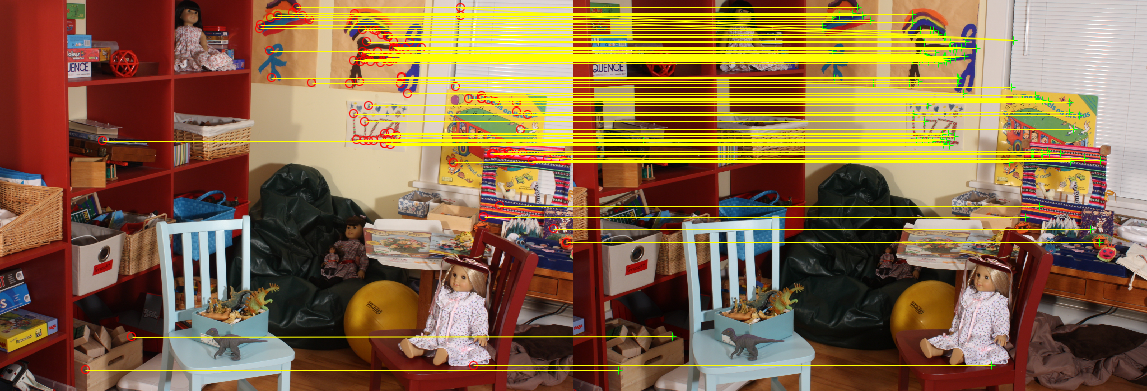
\includegraphics[width=\textwidth]{img/good_stereo}
		\caption{A subset of the matches found in this image pair.}\label{fig:good_stereo}
	\end{subfigure}
	\begin{subfigure}{\textwidth}
		\centering
		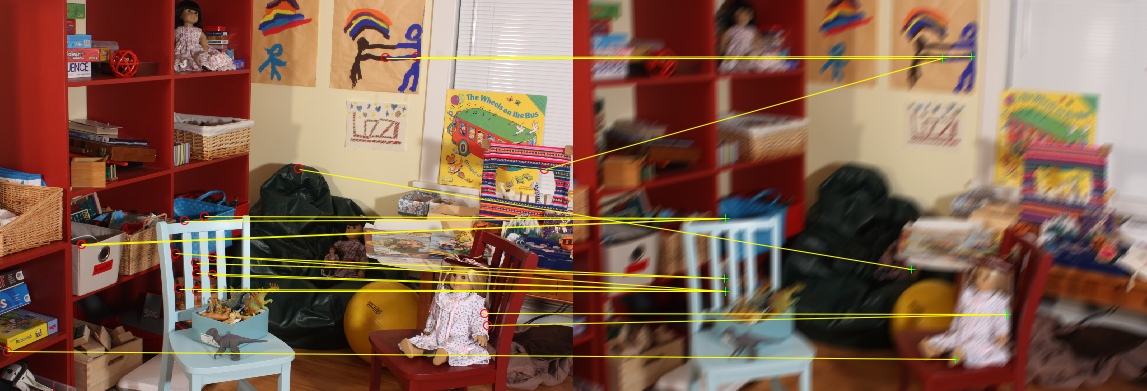
\includegraphics[width=\textwidth]{img/motion_blur}
		\caption{Motion blur reduces both the number and quality of matches.}\label{fig:motion_blur}
	\end{subfigure}
	\begin{subfigure}{\textwidth}
		\centering
		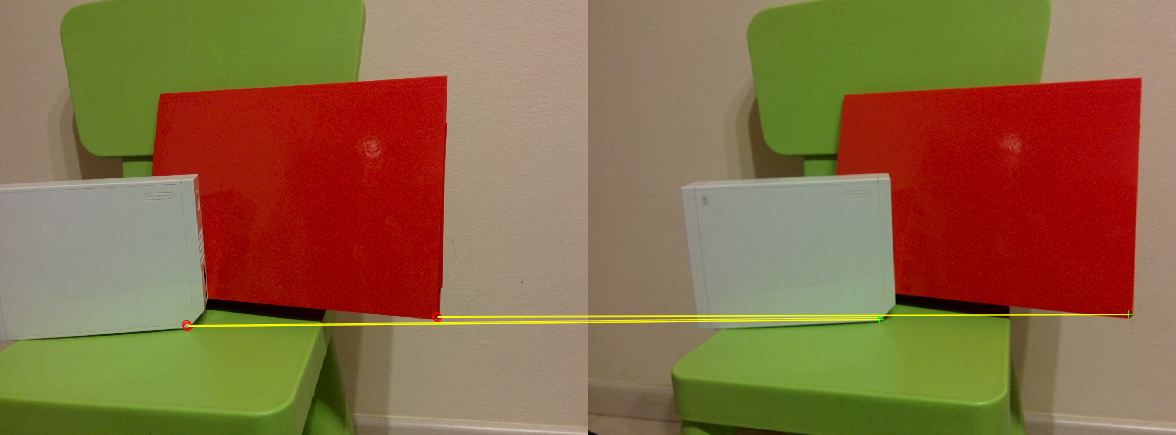
\includegraphics[width=\textwidth]{img/textureless_stereo}
		\caption{Textureless images provide few feature points.}\label{fig:textureless}
	\end{subfigure}
	\caption{Some examples of problems that may occur when matching correspondence search.}\label{fig:matching_problems}
\end{figure}

\subsection{Feature Detectors}
As we discussed in section~\ref{subsec:motion_estimation}, in order to estimate
the essential matrix, we need to find corresponding points in image pairs.
Typically, these points are called \textit{feature points} or \textit{keypoints}.
%
A feature point is an area in an image that is likely to be unique; i.e., it is a point of interest such as a corner.
%
Furthermore, for each feature point, we can extract some local information that describes it, this piece of information is called \textit{feature descriptor} and it is usually stored as a vector.
%
There are many different algorithm to extract feature points and descriptors such as the 
\emph{Moravec detector}~\cite{moravec1980obstacle}, the \emph{Harris
corner detector}~\cite{harris1988combined}, the
\emph{SIFT} keypoints detector and descriptor\cite{lowe1999object}, \emph{SURF} keypoints detector and descriptor\cite{bay2006surf}, etc.
%
Some of these feature points or descriptors can be affected by rotations and scale. Since SfM is based on many pictures taken from different views, SIFT features have always been 
preferred over other less robust features because of their rotational and scale
invariance. One of the main drawback is that SIFT is patented and can not be used freely as other detectors.
%
SURF~\cite{bay2006surf} is an alternative to SIFT that is also
rotational and scale invariant; SURF is patented too and 
can not be used for commercial applications but there is an available 
implementation in the MATLAB's Computer Vision Toolbox and it can be 
used for research.

Even though SIFT and SURF are some of the most used feature algorithms 
because of their robustness and invarince properties, there is little they can
do with poorly selected image pairs. Figure~\ref{fig:matching_problems} shows 
some of the most common problems that may arise from correspondence matching.
In general, the large variety of environments, each with its own characteristics, 
prevents a single technique to prevail over the others and this is one of 
the reason why a truly general-purpose SfM pipeline does not exists.
For a more detailed discussion about the differences amongst point detectors, 
see~\cite{schmidt2010evaluation, govender2009evaluation}.

\subsection{Outliers Rejection}
Since the motion estimation step is the core of SfM pipelines, its performance
affects the overall software; in particular, motion estimation is influenced 
by the presence of outliers in features matching.
A matching outlier is a pair of feature points that are erroneously considered 
corresponding points. If the motion estimation phase considered these points for
its computation, the result would be unreliable and it could compromise the 
whole camera's path estimation because of the incremental nature of the SfM 
pipeline.
In order to reduce this phenomenon, we can switch to a more robust feature points
detector and use a RANSAC approach to remove outliers before the motion estimation step.
RANSAC\cite{fischler1981random} is a model fitting algorithm for dataset that includes outliers.
This algorithm is iterative. At each iteration, it selects a subset of input data and computes the model based on this subset only. Then, RANSAC divides the complete dataset into a consensus set and outliers. If the number of outliers, computed thanks to a problem specific loss function, is
less than a given threshold, the estimated model is considered valid.

RANSAC is now a standard step in SfM. In this case, a certain number of correspondences is selected randomly, $E$ is computed 
according to the selected matches and the quality of the estimation is evaluated 
according to the reprojection error defined as
%
\begin{equation*}
	Err =  
	\sum_{i = 1}^N\sum_{j = 1}^n 
	d(K_iE\myvec{M}^j, \myvec{m}_i^j) \text{.}
\end{equation*}
%
This error formulation is similar to equation~\ref{eq:bundle_adj}, 
but now $E$ is not decomposed in $[R_i|\myvec{t}_i]$. The use of RANSAC before motion estimation provides a more reliable 
estimation even if the number of outliers is high (40-50\%).

\section{Full Spherical Cameras}
In the following sections we describe the full spherical photography's camera
model (section~\ref{subsec:spherical_camera_model}), the equirectangular image
format used to map spherical images on 2D matrix of pixels 
and the problems for SfM algorithms caused by this format 
(section~\ref{subsec:image_format}).
In section~\ref{subsec:related_work} we give an overview of the efforts of 
previous studies on this topics and describe the contribution of our work to 
this field.

\subsection{Spherical camera model}
\label{subsec:spherical_camera_model}
In Figure~\ref{fig:camera_model} we can see the full spherical camera model.
The axes' origin is also the center of projection. The image is formed on 
the unitary sphere whose center coincide with the center of projection.
$\myvec{m}$ is the projection on the sphere for the world point 
$\myvec{M}$, thus $\myvec{m}$ is a unitary vector that lies on the ray that goes
from the center of projection to the point $\myvec{M}$.
The image point $\myvec{m}$ is defined by the spherical coordinate 
system composed of the two angles $\lambda$ and $\phi$, that represent the 
longitude and latitude respectively. 
We can use the following formula to convert the spherical coordinates to 
euclidean:
\begin{equation}
	\label{eq:ll2Cartesian_second}
	\myvec{m} =
	\begin{pmatrix}
		\cos\phi\sin\lambda \\
		-\sin\phi \\
		\cos\phi\cos\lambda
	\end{pmatrix}	\text{.}
\end{equation}
Since this model is essentially different from the 
perspective camera's~\cite{szeliski2010computer}, the traditional procedures 
for pose estimation of the computer vision frameworks can not be used.
We show in section~\ref{sec:keypoints_conversion} how we can still exploit
equation~\ref{eq:epipolar_equation} to estimate the essential matrix and use it
to compute the camera motion.
\begin{figure}[h]
    \centering
    \def\svgwidth{0.7\columnwidth}
    \input{img/coordinate_system.pdf_tex}
    \caption{Full spherical camera model.}
	\label{fig:camera_model}
\end{figure}

\subsection{Equirectangular Image Format}
\label{subsec:image_format}
The equirectangular image format (Figure~\ref{fig:equirectangular}) is a 2D
representation for omnidirectional 
images. It stores each 3D image points in a bidimensional matrix of pixels
by mapping the two angular dimensions (latitude and longitude) to the two
linear dimensions of the image (height and width); latitude increases from 
top to bottom while longitude increases from left to right.
In particular, the equirectangular mapping for a full spherical images is the
following:
\begin{subequations}
	\label{eq:ll2Cartesian_first}
	\begin{align}
	\lambda &= \frac{u}{W 2 \pi} - \pi \\
	\phi &= \frac{\pi}{2} - \frac{v}{H \pi}\text{,}
	\end{align}
\end{subequations}
\noindent where \textit{W} and \textit{H} are, respectively, 
the image's width and height while $u$ and $v$ are the pixel coordinate 
in the equirectangular image, like in figure~\ref{fig:equirectangular}.
In case of full spherical images, we have that
$ \lambda \in [-\pi; \pi] $ and $\phi \in [-\frac{pi}{2}; \frac{pi}{2}] $.

The equirectangular format introduces significant distortions, especially 
around the poles; this compromises the robustness of the feature matching 
procedure which can then return incorrect estimations for the essential 
matrix.
Similarly to the feature matching issue, distortions causes particular problems
with the block-matching algorithms for disparity map computation.
In Section~\ref{sec:pipeline_densification} we describe the modified 
block-matching procedure we designed to reduce the effect of distortions 
when computing disparity maps.
\begin{figure}[h]
	\centering
	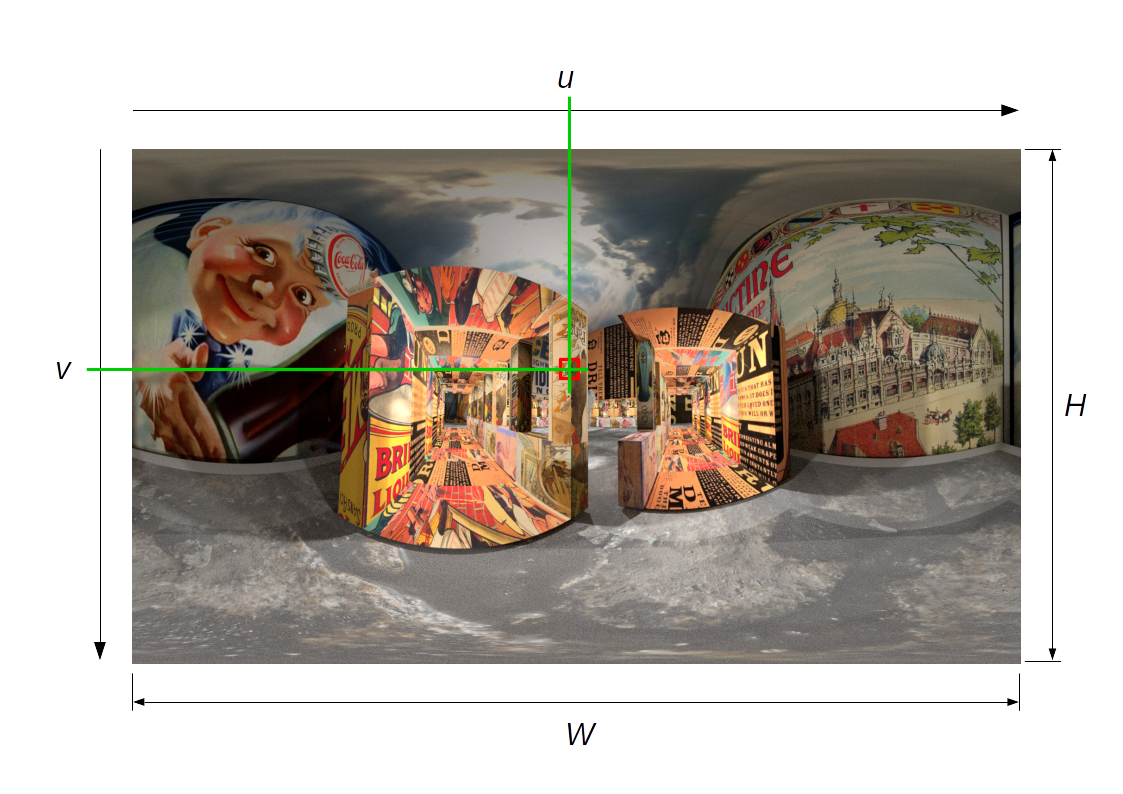
\includegraphics[width=0.8\textwidth]{img/equirectangular}
	\caption{The equirectangular image format maps the 3D image points in 
	spherical coordinates to the 2D image point $(u, v)$.}
	\label{fig:equirectangular}
\end{figure}

\subsection{Previous Work on Spherical SfM}
\label{subsec:related_work}
As we pointed out in the previous sections, there has been few research 
effort to use full spherical cameras in SfM and most of the work
has targeted perspective cameras.
Most of the work about panoramic cameras has employed catadioptric or dioptric 
devices with single image sensor (no stitching), therefore, as we said in 
section~\ref{sec:cameraclassification}, none of this types of camera is capable
to produce full spherical images.

In~\cite{li2008binocular,li2006real}, Li developed a rectification procedure for wide
FOV cameras that enables the computation of disparity maps with standard 
block-matching algorithms; the rig he used for testing was composed of 
fisheye cameras that could not provide full spherical views.
Ma et al. in~\cite{ma20153d} used equirectangular images produced with a 
RICO THETA S to create disparity maps. They manually selected some 
correspondences in order to compute the essential matrix correctly and then 
used the epipolar geometry to remove correspondences outliers after an 
automatic feature matching step. Because of the user intervention in 
the pipeline, they could not test their results on long sequences, moreover the
computed disparity were noisy.
On the contrary, Arican et al.~\cite{arican2007dense} developed a new algorithm
based on graph-cut to compute disparities for omnidirectional images directly.
They obtained high quality disparity maps with thanks to their new method.
Im et al.~\cite{im2016all} focused on the creation of a framework to produce
depth maps 
with full spherical consumer devices. They focused on short video sequences 
with small motion of the camera as input data.
Aly et al.~\cite{aly2012street} extracted the interest points' directions from the
equirectangular 
images with Equation~\ref{eq:ll2Cartesian_second} and then used the 
epipolar equation (\ref{eq:epipolar_equation}) to estimate the essential matrix.
Their work focused only on pose estimation from an unordered set of images
and they assumed the camera movements were constrained to a plane.
In~\cite{kangni2007orientation}, Kangni et al. converted the full spherical image format to 6 
separate perspective projection on the faces of a cube around the viewer; 
then they used the epipolar equation to obtain the essential matrix;
they focused on motion estimation without dense reconstruction.
%\todo[inline]{citare Arican e Densificazione di Pagani}
Pagani et al.~\cite{pagani2011structure} designed an SfM pipeline for full
spherical cameras that exploits spherical coordinates directly (without 
reprojecting the 3D directions on a planar image). They focused their studies on
the effect of the different error metrics for pose estimation and provided a 
sparse reconstruction and pose estimation algorithm.

In this work we propose a complete SfM pipeline with dense point cloud 
reconstruction for 360\degree video sequences with the following 
characteristics:
\begin{itemize}
	\item no view selection is needed, i.e. it works with every frame of the 
	input video sequence by automatically discarding the unnecessary images;
	\item the pose estimation is based on the 2D-to-2D approach
	(see section~\ref{subsec:motion_estimation}) and it uses both frontal and
	backward hemisphere's correspondences;
	\item it employs a novel block-based disparity estimation algorithm that 
	reduces the matching problems caused by the
	typical distortions of equirectangular images;
	\item it provides a dense point cloud as an estimation of the environment.
\end{itemize}
Our contribution includes:
\begin{itemize}
	\item the development of the frame selector that chooses the images to be
	used for motion estimation among all the video's frames;
	\item the adaptive block-matching algorithm for disparity maps with 
	equirectangular images;
	\item the entire implementation of our SfM pipeline in MATLAB.
\end{itemize}.
